\section{Otimização}


\marcador{subsection}{Extremos locais}
\begin{definb}{}{}
\begin{enumerate}
\item Dizemos que uma função $f$ de duas variáveis tem um \dt{valor máximo local} no ponto
{\color{red}$(a,b)$} se existir  uma bola aberta $B_r({\color{red}a,b})$ tal que {\color{blue}$f({\color{red}a,b})\geq f(x,y)$} para todo $(x,y)\in B_r({\color{red}a,b})$.

\item Dizemos que uma função $f$ de duas variáveis tem um \dt{valor mínimo local} no ponto
{\color{red}$(a,b)$} se existir  uma bola aberta $B_r({\color{red}a,b})$ tal que
{\color{blue}$f({\color{red}a,b})\leq f(x,y)$ } para todo
$(x,y)\in B_r({\color{red}a,b})$.
\end{enumerate}
\end{definb}

\begin{center}
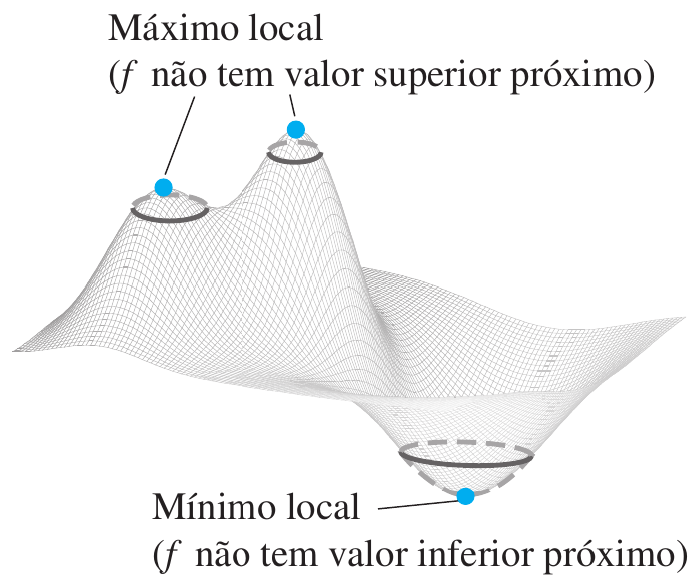
\includegraphics[scale=.7]{figuras/ext-local.png}
\end{center}
\newpage

\marcador{subsection}{Pontos críticos}
\begin{theoremb}{}{}
Se $f(x,y)$ tem um extremo local em {\color{red}$(a,b)$} e possui derivadas parciais em
{\color{red}$(a,b)$}, então
\[\nabla f({\color{red}a,b})=0.\]
\end{theoremb}

Um ponto {\color{red}$(a,b)$} tal que $\nabla f({\color{red}a,b})$ não existe ou $\nabla f({\color{red}a,b})=0$   é
dito \dt{ ponto crítico ou ponto estacionário} de $f$.

\begin{exeb}{}{}
Determine os  pontos críticos de
\begin{enumerate}
\item $f(x,y)=x^2+y^2-2x-6y+14$

\item \(f(x,y)=y^2-x^2\)
\end{enumerate}
\end{exeb}
\newpage

\marcador{subsection}{Teste da Segunda Derivada}
%\begin{scriptsize}

Se $f$ é uma função de duas variáveis com todas as derivadas de ordem 2 no ponto ${\color{red}(a,b)}$, definimos
\[D^2f({\color{red}a,b})=
\left[\begin{array}{cc}
f_{xx}({\color{red}a,b}) & f_{xy}({\color{red}a,b})\\
\\
f_{yx}({\color{red}a,b}) & f_{yy}({\color{red}a,b})
\end{array}   \right],\]
chamada \dt{matriz Hessiana} da função $f$ no ponto $({\color{red}a,b})$.

\begin{theoremb}{Teste da Segunda Derivada}{}

Seja $z=f(x,y)$ uma {\color{blue}função de classe $C^2$} em uma bola $B_r({\color{red}a,b})$ tal que $\nabla f({\color{red}a,b})=(0,0)$. Neste caso,
\begin{enumerate}[(a)]
\item Se $\det D^2f({\color{red}a,b}){\color{blue}>0}$ e
$f_{xx}({\color{red}a,b}){\color{red}<0}$, então $({\color{red}a,b})$ é
{\color{red}máximo local}.

\item Se $\det D^2f({\color{red}a,b}){\color{blue}>0}$ e
 $f_{xx}({\color{red}a,b}){\color{blue}>0}$, então $({\color{red}a,b})$
é {\color{blue}mínimo local.}

\item Se $\det D^2f({\color{red}a,b}){\color{red}<0}$, então $({\color{red}a,b})$ é {\color{red}ponto de sela}.
\end{enumerate}
\end{theoremb}

\begin{caixavermelha}{}
\begin{center}
Se $\det D^2f(a,b)=0$, nada podemos concluir.
\end{center}
\end{caixavermelha}

\begin{exeb}{}{}
Localize e classifique os pontos críticos de $f(x,y)=x^4+y^4-4xy+1$.
\end{exeb}
 \begin{minipage}{0.5\textwidth}
 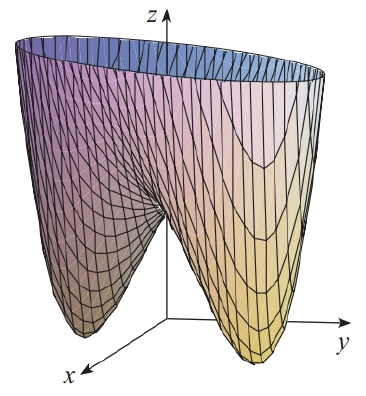
\includegraphics[scale=.7]{figuras/teste-derv2.png}
 \begin{center}
 \end{center}
 \end{minipage}
  \begin{minipage}{0.2\textwidth}
  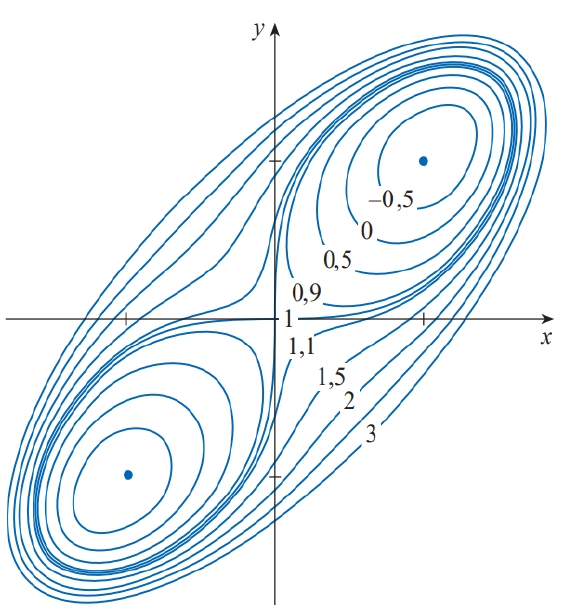
\includegraphics[scale=.6]{figuras/mapa-cont.png}
  \end{minipage}


\marcador{subsection}{Extremos Globais}
\begin{definb}{}{}
Seja uma função $f$ de duas variáveis definida em um conjunto $U\subset \R^2$.
\begin{enumerate}
\item Dizemos que $f$  tem um valor \dt{máximo absoluto} em $U$ se existir um ponto $(a,b)\in U$ tal que $f(a,b)\geq f(x,y)$ para todo $(x,y)\in U$. Neste caso, $f(a,b)$ é {\color{red} o valor máximo absoluto }de $f$ em $U$.

\item Dizemos que $f$  tem valor \dt{mínimo absoluto} em $U$ se existir um ponto $(a,b)\in U$ tal que $f(a,b)\leq f(x,y)$ para todo $(x,y)\in U$. Neste caso, $f(a,b)$ é {\color{red}o valor mínimo absoluto} de $f$ em $U$
\end{enumerate}
\end{definb}

\begin{exeb}{}{}
\begin{enumerate}
\item A função  $f(x,y)=1-x^2-y^2$ tem máximo absoluto em $\R^2$ no ponto $(0,0)$.

\item A função $f(x,y)=x$ não tem máximo nem mínimo absoluto em $\R^2$.
\end{enumerate}
\end{exeb}
\newpage

\marcador{subsection}{Topologia no plano}

Antes de enunciarmos nosso próximo resultado, precisamos de algumas noções topológicas no plano.


\begin{itemize}
\item Um conjunto é dito {\color{orange}limitado} se ele está contido em algum disco.

\item A \dt{fronteira} de um conjunto $D$, denotada por $\partial D$, é formada por pontos $(a,b)$ tais que qualquer disco aberto com centro em $(a,b)$ contém pontos de $D$ e pontos que não estão em $D$.


\item Um conjunto $D$ de $\R^2$ é dito \dt{fechado} se contém todos os pontos de sua fronteira, onde

\item Um conjunto \dt{fechado} e {\color{orange}limitado} é dito ser \dt{compacto}.

\item Um conjunto  é {\color{red} aberto} quando seu complementar é fechado.


\end{itemize}

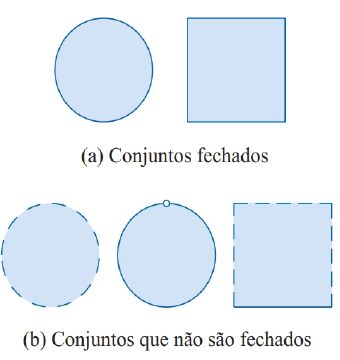
\includegraphics[scale=1]{figuras/fechados.png}


\newpage

\begin{theoremb}{Teorema de Weierstrass}{}
Se $f$ é uma {\color{red}função contínua} definida em um {\color{red}conjunto fechado e limitado} $D$ então $f$ {\color{blue}assume valor máximo e mínimo absolutos} em $U$.
\end{theoremb}

\begin{caixaazul}{Determinação de Extremos Absolutos}{}
Para determinarmos os extremos absolutos de uma {\color{red}função contínua} definida em um {\color{red}conjunto fechado e limitado} $D$:
\begin{enumerate}
\item Determinar os valores de $f$ nos pontos críticos de $f$ em $D$.
\item Determinar os valores extremos de $f$ na fronteira de $D$.
\item O maior dos valores dos passos anteriores será o máximo absoluto e o menor deles o valor mínimo absoluto.
\end{enumerate}
\end{caixaazul}

\begin{exeb}{}{}
Determine os valores extremos da função $f(x,y)=2+2x+2y-x^2-y^2$ na região triangular no primeiro quadrante limitada pelas retas \(x=0, y=0, y=9-x\).
\end{exeb}






